% vim:ft=tex
% rubber: module xelatex

\subsection{Stereo matching}
\label{sec:stereo}
We have implemented dynamic programming based stereo matching using the methods
described by \citet{realtimestereo}. The output of the stereo matching is a
disparity map for each of the left and right images; the disparity map is a grey
scale image with black (or 0) signifying the lowest disparity, and white (or
255) signifying the maximum disparity. The disparity map is built using a
dynamic programming matrix for each scan line in the image; in the simplest
case, the process is as follows (for each scan line):

\begin{enumerate}
\item Create the dynamic programming matrix, $A$, with width and height both
  equal to the length of the scan line (i.e. the width of the images).
  Initialise the top-left corner to 0.

\item Step through the matrix, calculating $A[i,j] = \mathrm{min}(A[i-1,j],
  A[i,j-1], A[i-1,j-1]) + \mathrm{diff}(\mathrm{imageL}[i], \mathrm{imageR}[j])$
  where \texttt{diff} gets the difference between the image pixel values in the
  current scan line.

\item Calculate the path of minimal cost through the matrix $A$, starting in the
  bottom right corner, and moving from there to the adjacent position with the
  minimum value, i.e. $\mathrm{min}(A[i-1,j], A[i,j-1], A[i-1,j-1])$. Fill the
  disparity map with the appropriate value ($\mathrm{DisparityMapL}[i,y]=j-i$,
  $\mathrm{DisparityMapR}[j,y]=i-j$).
\end{enumerate}

After having built up the disparity maps for the entire image (i.e. after doing
the above for all scan lines), go through them and normalise the values to the
range $[0,255]$, or alternatively multiply the matrices by a user-configurable
factor.

In addition to the simple version of the disparity mapping algorithm described
above, we have implemented the following (optional) modifications, in order to
improve the quality of the matching:

\begin{enumerate}
\item It is possible to assign an additional bonus or penalty to moving
  diagonally in the dynamic programming matrix, depending on whether we want
  smooth or spiky (very disparate) images respectively.

\item The choices for each scan line can be modified by those for the previous
  scan line, reducing error by ``suggesting'' ways to conform. We suggest a factor
 of \~0.5 as standard.

\item A median filter can be applied to the stereo images before building the
  disparity map, to get rid of noise.

\item It is possible to step through the dynamic programming matrix not only from
  the bottom-right to top-left corner, but also from top-left to bottom-right,
  and then choose the least-weight path overall. This helps reduce the cases
  where one of them goes horribly off the 'best' path because it, intuitively,
  followed the lowest-weight path into a dead end. We use this double-processing
 by default.

\item The running time can be improved by selecting a maximum disparity bound,
  $b$. The ``path of least resistance'' is never allowed to go outside this
  disparity bound because we set $A[i,j]$ to a vast positive value if $i > b$ or
  $j > b$.
\end{enumerate}


%%% Leaving this out for now...
% One improvement we didn't implement: line skipping. (In that version, at
% thebeginning, every n’th horizontal line is calculated to find bounding space
% for possible disparities in between.)


\subsubsection{Testing of stereo matching}

\begin{figure}[p]
  \centering
  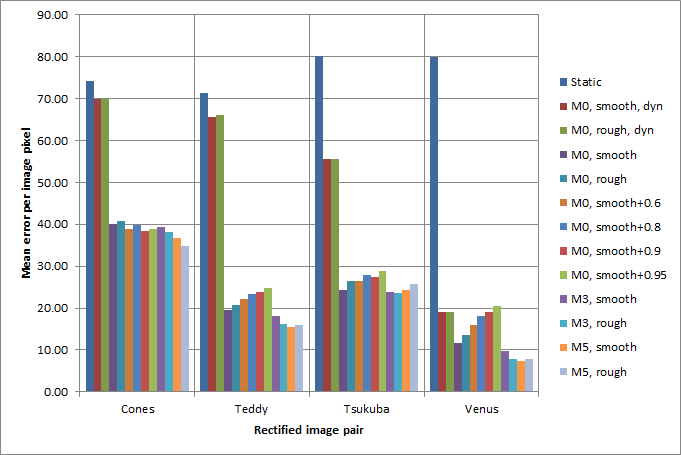
\includegraphics[height=0.4\textheight]{Stereo-left-report}\\[2mm]
  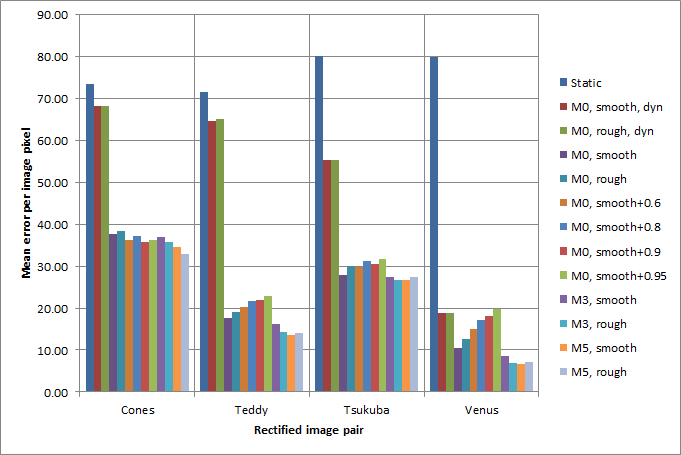
\includegraphics[height=0.4\textheight]{Stereo-right-report}
  \caption[Results of stereo matching]{Results of stereo matching for the left
    (top graph) and right (bottom graph) images, using various parameters.
    Resulting depth maps are compared to the canonical depth maps to obtain
    discrepancies (quantities of error). Each coloured column in the chart is a
    different parameterisation, as tested on one of the four images. `Static' is
    the baseline difference between the canonical depth map and a image with
    randomised values. `M0' indicates a median filter was not used in
    preprocessing. `M3' and `M5' indicate median filters of size 3 and 5
    respectively. `rough' indicates scanlines did not influence each other.
    `smooth' indicates each scanline was influenced by the one previous, by 0.5
    by default or by the amount given. `dyn' indicates the depth map was created
    by stretching the disparities to the full [0...255] range, instead of
    multiplying by the value recommended by \cite{middlebury} for each
    particular image.}
  \label{fig:stereo-report}
\end{figure}

See figure~\ref{fig:stereo-report}. Our stereo matching algorithm, while rather
hit-and-miss, constructs recognisable depth maps. The quality of the results is
rather dependent on the specific parameters used. We should note that in some
cases, the output `looks better' (e.g. is more coherent or shaded) even if it is
strictly less accurate.

We took the best results and submitted them to the Middlebury online tests.
\cite{stereocorrespondence, middlebury} Their calculator unfortunately
presupposes a cyclopean image, which we were not calculating. We submitted left
and right instead, and chose the better of the two in each case. Still, we
expect we would have scored considerably higher if we had calculated the
cyclopean images. However, the details of our implementation made this
difficult.

We had 44.9\% to 45.8\% bad pixels total. The worst Middlebury have on record is
20.7\%. \cite{stereocorrespondence, middlebury} For our test disparity maps,
`Tsukuba' was best with 17.9\% error. `Venus' and `Teddy' were mediocre with
40.5\% and 54.4\% respectively. `Cones' was worst with 69.0\%. See
figure~\ref{fig:stereo-report} for full details.

\begin{figure}[p]
 \centering

 \subfloat[Tsukuba (rough)] { \label{fig:tsu-1} 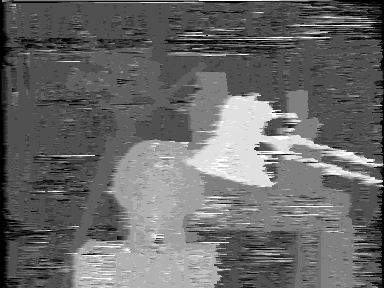
\includegraphics[trim = -2mm -2mm -2mm -2mm, width=0.23\textwidth]{stereo/tsu_imL_mat0_hardmult} }
 \subfloat[Venus (rough)] { \label{fig:ven-1} 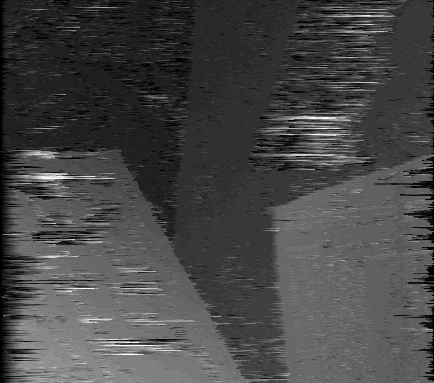
\includegraphics[trim = -2mm -2mm -2mm -2mm, width=0.23\textwidth]{stereo/ven_imL_mat0_hardmult} }
 \subfloat[Cones (rough)] { \label{fig:con-1} 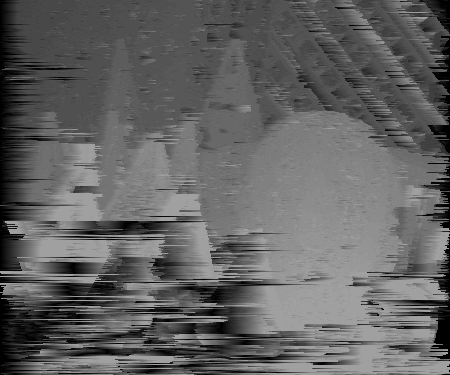
\includegraphics[trim = -2mm -2mm -2mm -2mm, width=0.23\textwidth]{stereo/con_imL_mat0_hardmult} }
 \subfloat[Teddy (rough)] { \label{fig:ted-1} 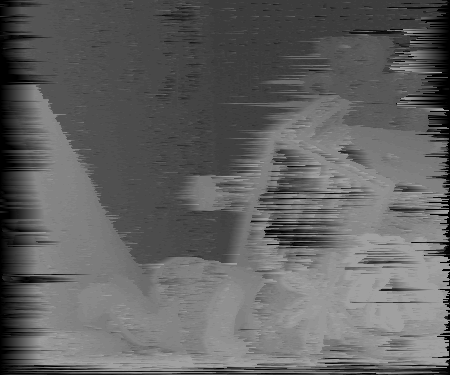
\includegraphics[trim = -2mm -2mm -2mm -2mm, width=0.23\textwidth]{stereo/ted_imL_mat0_hardmult} }\\

 \subfloat[Tsukuba (mid)] { \label{fig:tsu-2} 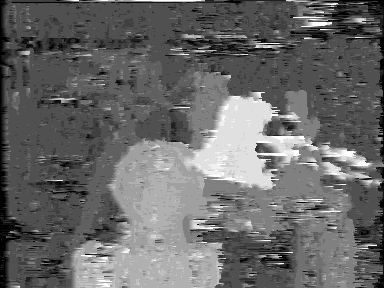
\includegraphics[trim = -2mm -2mm -2mm -2mm, width=0.23\textwidth]{stereo/tsu_imL_mat5_hardmult_smooth} }
 \subfloat[Venus (mid)] { \label{fig:ven-2} 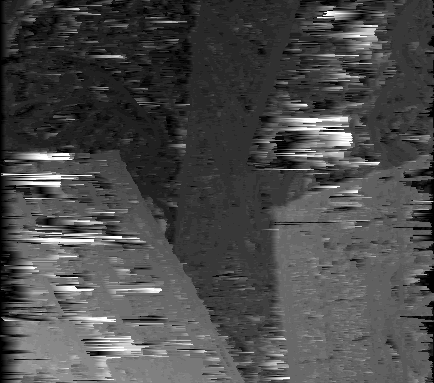
\includegraphics[trim = -2mm -2mm -2mm -2mm, width=0.23\textwidth]{stereo/ven_imL_mat5_hardmult_smooth} }
 \subfloat[Cones (mid)] { \label{fig:con-2} 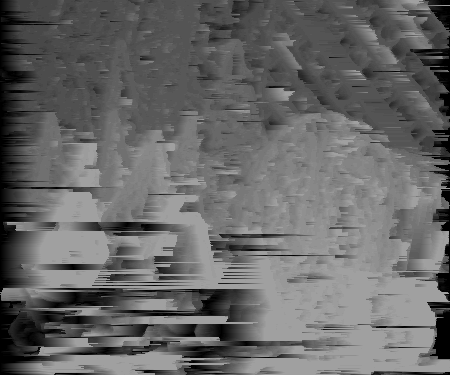
\includegraphics[trim = -2mm -2mm -2mm -2mm, width=0.23\textwidth]{stereo/con_imL_mat5_hardmult_smooth} }
 \subfloat[Teddy (mid)] { \label{fig:ted-2} 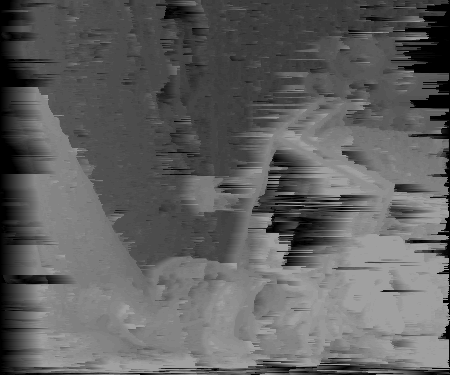
\includegraphics[trim = -2mm -2mm -2mm -2mm, width=0.23\textwidth]{stereo/ted_imL_mat5_hardmult_smooth} }\\

 \subfloat[Tsukuba (smooth)] { \label{fig:tsu-4} 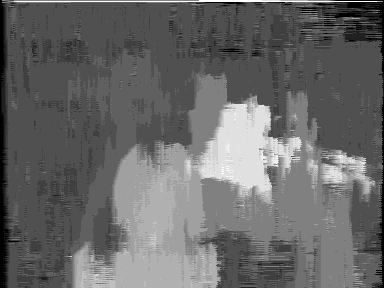
\includegraphics[trim = -2mm -2mm -2mm -2mm, width=0.23\textwidth]{stereo/tsu_imL_mat0_hardmult_smooth0.9.png} }
 \subfloat[Venus (smooth)] { \label{fig:ven-4} 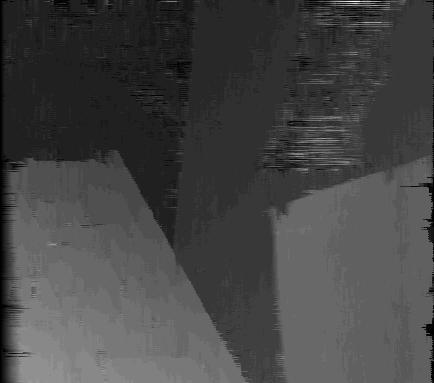
\includegraphics[trim = -2mm -2mm -2mm -2mm, width=0.23\textwidth]{stereo/ven_imL_mat0_hardmult_smooth0.9.png} }
 \subfloat[Cones (smooth)] { \label{fig:con-4} 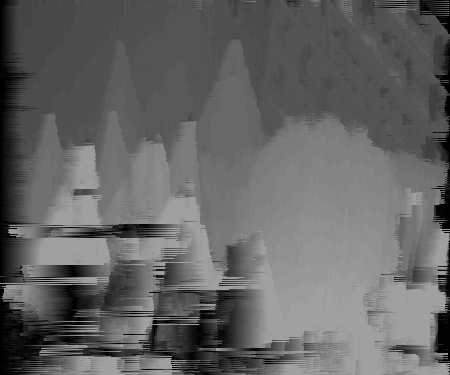
\includegraphics[trim = -2mm -2mm -2mm -2mm, width=0.23\textwidth]{stereo/con_imL_mat0_hardmult_smooth0.9.png} }
 \subfloat[Teddy (smooth)] { \label{fig:ted-4} 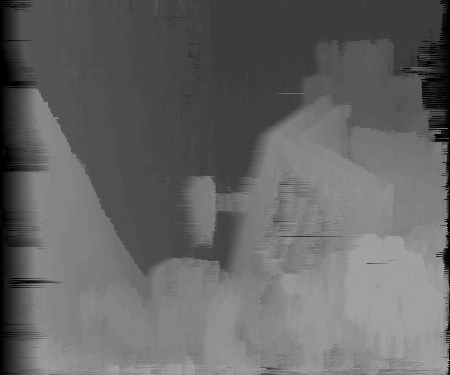
\includegraphics[trim = -2mm -2mm -2mm -2mm, width=0.23\textwidth]{stereo/ted_imL_mat0_hardmult_smooth0.9.png} }

 \subfloat[Tsukuba (ideal)] { \label{fig:tsu-i} 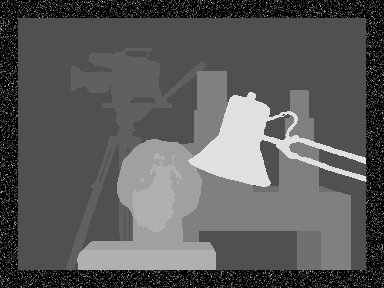
\includegraphics[trim = -2mm -2mm -2mm -2mm, width=0.23\textwidth]{stereo/tsu_ideal_L} }
 \subfloat[Venus (ideal)] { \label{fig:ven-i} 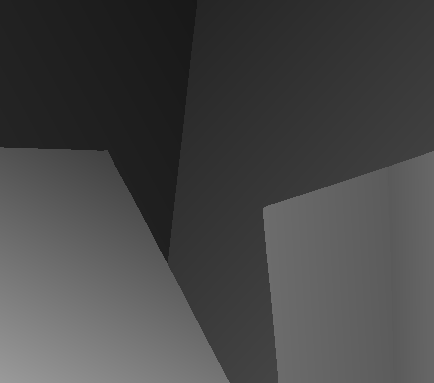
\includegraphics[trim = -2mm -2mm -2mm -2mm, width=0.23\textwidth]{stereo/ven_ideal_L} }
 \subfloat[Cones (ideal)] { \label{fig:con-i} 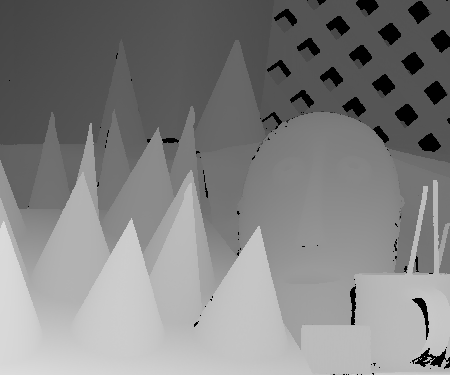
\includegraphics[trim = -2mm -2mm -2mm -2mm, width=0.23\textwidth]{stereo/con_ideal_L} }
 \subfloat[Teddy (ideal)] { \label{fig:ted-i} 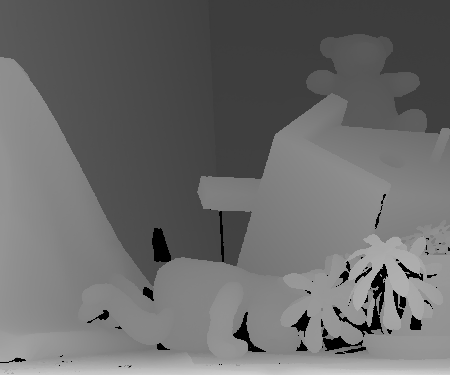
\includegraphics[trim = -2mm -2mm -2mm -2mm, width=0.23\textwidth]{stereo/ted_ideal_L} }\\

 \caption[Examples of dynamic programming with various parameters]{Examples of
   dynamic programming with various parameters. Canonical baseline images are
   courtesy of \citet{stereocorrespondence}. `rough' images are not
   preprocessed. `mid' images have a 5x5 median filter applied in preprocessing
   and feature inter-scanline smoothing with a weight of 0.5. `smooth' images
   feature inter-scanline smoothing with a weight of 0.9.}
 \label{fig:stereo-image-depth-maps}
\end{figure}

\begin{figure}[p]
 \centering
 \subfloat[Depth map (no smoothing)] { \label{fig:sm-1} 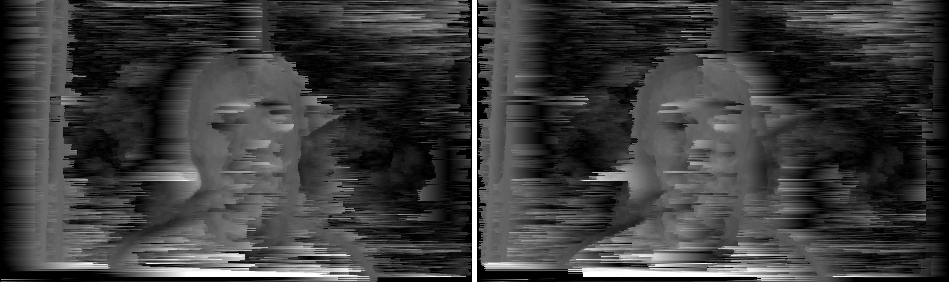
\includegraphics[trim = -2mm -2mm -2mm -2mm, width=0.8\textwidth]{stereo/lowsmooth} }\\
 \subfloat[Depth map (low smoothing)] { \label{fig:sm-2} 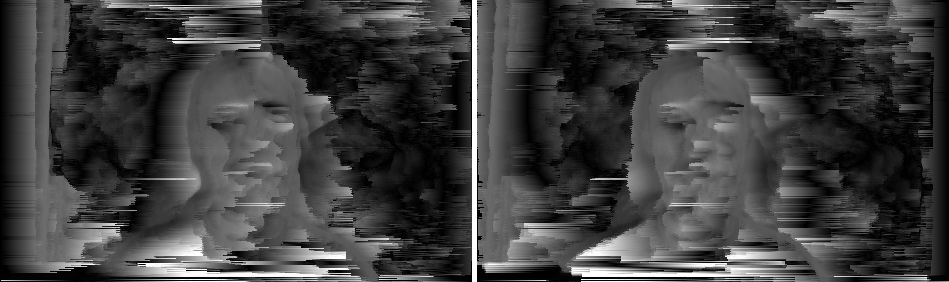
\includegraphics[trim = -2mm -2mm -2mm -2mm, width=0.8\textwidth]{stereo/midsmooth} }\\
 \subfloat[Depth map (mid smoothing)] { \label{fig:sm-3} 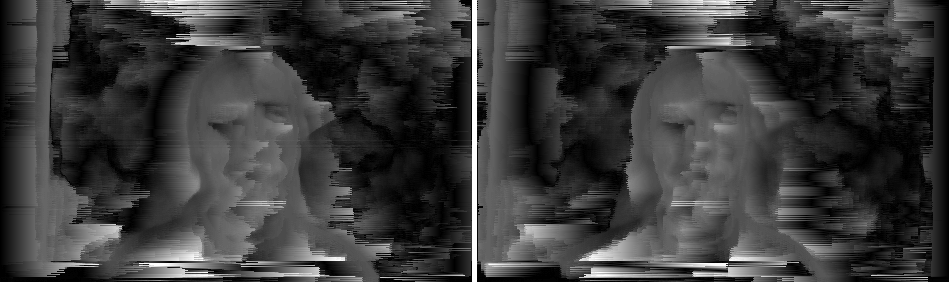
\includegraphics[trim = -2mm -2mm -2mm -2mm, width=0.8\textwidth]{stereo/highsmooth} }\\
 \subfloat[Depth map (high smoothing)] { \label{fig:sm-4} 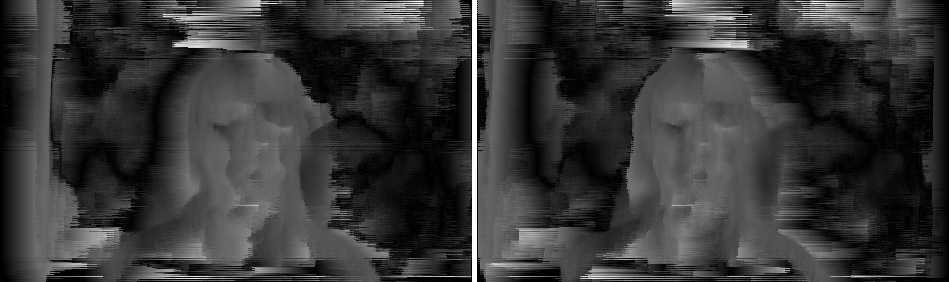
\includegraphics[trim = -2mm -2mm -2mm -2mm, width=0.8\textwidth]{stereo/extremesmooth} }
 \caption[Depth maps for stereo pairs created with various parameters]{Depth
   maps for one of the stereo pairs in our database, calculated using increasing
   levels of smoothness.}
 \label{fig:stereo-pair-depth-maps}
\end{figure}

Consider Figure~\ref{fig:stereo-pair-depth-maps}. Increasing the three
smoothness parameters - median matrix size, inter-scanline smoothing, and
diagonal preference / disparity penalty - often results in less noise, but loss
of definition. This can sometimes translate to poorer performance on the
formal tests, even when it makes the images more human-readable.
